\documentclass[../../main.tex]{subfiles}
\begin{document}
\rhead{京都大学後期$1995$年$6$番}
\setcounter{equation}{0}
\begin{oframed}
  \subfile{problem}
\end{oframed}
\setlength{\columnseprule}{0.4pt}
\begin{multicols}{2}
  {\bf [解答]}
  \paragraph{(1)}

  \begin{figure}[H]
    \centering
    \begin{tikzpicture}[x=1.1cm,y=1.25cm,>=stealth,
      every node/.style={font=\small}]
      % a=3/2 の例．M は L_a と RQ の交点で，接点とは異なる．
      \pgfmathsetmacro{\aval}{1.5}
      \pgfmathsetmacro{\xm}{4*\aval*(2-\aval)/(8-\aval*\aval)}
      \pgfmathsetmacro{\ym}{4*(4-\aval)/(8-\aval*\aval)}
      \coordinate (O) at (0,0);
      \coordinate (Q) at (0,2);
      \coordinate (R) at (4,0);
      \coordinate (A) at (\aval,0);
      \coordinate (B) at (0,{4/\aval});
      \coordinate (M) at (\xm,\ym);
      \fill[pattern=north east lines,pattern color=blue!60]
      (O) -- (A) -- (M) -- (Q) -- cycle;
      \draw[->,thick,gray!80!black] (-0.15,0) -- (4.55,0) node[right] {$x$};
      \draw[->,thick,gray!80!black] (0,-0.15) -- (0,3.25) node[above] {$y$};
      \draw[very thick,blue!85!black,domain=0.35:4.3,samples=80]
      plot (\x,{1/\x});
      \draw[very thick,red!85!black] (Q) -- (R);
      \draw[very thick,teal!85!black] (B) -- (A);
      \draw[densely dotted,thick,gray!70!black]
      (M) -- (\xm,0) (M) -- (0,\ym);
      \foreach \p/\pos in {O/below left,R/below,A/below,B/above left,M/above right}{
        \node[circle,fill=blue!85!black,inner sep=1.2pt] at (\p) {};
        \node[\pos=2pt] at (\p) {$\p$};
      }
      \node[circle,fill=blue!85!black,inner sep=1.2pt] at (Q) {};
      \node[above left=2pt] at (Q) {$Q$};
      \node[below] at (\xm,0) {$x_0$};
      \node[left=10pt] at (0,\ym) {$y_0$};
      \node[blue!85!black,below right] at (2.5,0.4) {$y=1/x$};
      \node[red!85!black,above right] at (3.0,0.5) {$RQ$};
      \node[teal!85!black,right] at (1.0,1.0) {$L_a$};
    \end{tikzpicture}
    \caption{直線$RQ$と接線$L_a$の交点$M$．斜線部が$T$}
    \label{1995-6:fig:1}
  \end{figure}

  $x=t\,(t>0)$の$C$の接線は
  \begin{align}
    y=-\dfrac{1}{t^2}x+\dfrac{2}{t} \label{eq:1}
  \end{align}
  である．
  これが$A$を通る時，
  \begin{align}
    & 0 = -\dfrac{1}{t^2}a+\dfrac{2}{t}      \\
    \therefore
    & t = \dfrac{a}{2} \quad (\because t>0)
  \end{align}
  を満たすから，
  \cref{eq:1}に代入して
  \begin{align}
    L_a : y
    & = -\dfrac{4}{a^2}x+\dfrac{4}{a}
  \end{align}
  である．

  次に，直線RQの方程式は
  \begin{align}
    & RQ:y=-\dfrac{1}{2}x+2  \label{eq:2}
  \end{align}
  と表せるから，RQと$L_a$の交点の$x$座標$x_0$は
  \begin{align}
    & -\dfrac{4}{a^2}x_0+\dfrac{4}{a} = -\dfrac{1}{2}x_0+2 \\
    \therefore
    & (\dfrac{1}{2}-\dfrac{4}{a^2})x_0 = 2-\dfrac{4}{a}
  \end{align}
  の解である．$a \neq 2\sqrt{2}$のもとでこれを解いて
  \begin{align}
    x_0
    & = \dfrac{2-4/a}{1/2-4/a^2}                    \\
    & = \dfrac{4a(a-2)}{a^2-8}  \label{eq:3}
  \end{align}
  を得る．この時$y$座標は
  \begin{align}
    y_0  =  \dfrac{4(a-4)}{a^2-8}  \label{eq:4}
  \end{align}
  である．

  従って，$0<a<4$および$a \neq 2\sqrt{2}$のもとで，
  題意の条件は
  \begin{align}
    \begin{dcases}
      x_0 > 0 \\
      y_0 > 0
    \end{dcases}             \\
    \therefore
    \begin{dcases}
      \dfrac{4a(a-2)}{a^2-8} > 0 \\
      \dfrac{4(a-4)}{a^2-8} > 0
    \end{dcases} \\
    \therefore
    0 < a < 2
  \end{align}
  である．$\cdots$(答)

  \paragraph{(2)}
  (1)で求めた条件$0<a<2$のもとでとかんがえる．
  $T,S_1,S_2$は
  \begin{align}
    T+S_1 & = \triangle ORQ = \dfrac{1}{2} \cdot 2 \cdot 4 = 4           \\
    T+S_2 & = \triangle OAB = \dfrac{1}{2} \cdot a \cdot \dfrac{4}{a} = 2
  \end{align}
  と書けるから，
  $S_1 = 4-T$, $S_2 = 2-T$なので，$r$および$m$は$T$を用いて
  \begin{align}
    r
    & = S_1+S_2                     \\
    & = (4-T)+(2-T)                 \\
    & = 6-2T    \label{eq:5} \\
    m
    & = S_1S_2                      \\
    & = (4-T)(2-T)
  \end{align}
  となる．
  ここから$T$を除去して
  \begin{align}
    m
    & = \dfrac{1}{4}(r+2)(r-2)                  \\
    & = \dfrac{1}{4}(r^2-4) \label{eq:6}
  \end{align}
  である．

  \begin{figure}[H]
    \centering
    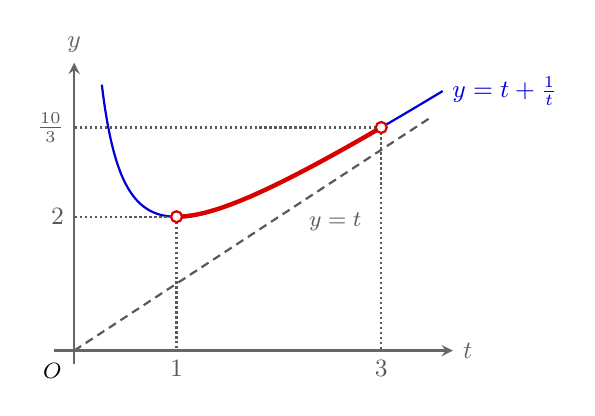
\begin{tikzpicture}[x=1.3cm, y=0.85cm, >=stealth,
      every node/.style={font=\small}]
      \coordinate (P) at (1, 2);
      \coordinate (R) at (3, {10/3});
      % 漸近線 y = t
      \draw[densely dashed, thick, gray!70!black, domain=0:3.5] plot (\x, \x);
      \node[below right=0pt, font=\footnotesize, gray!70!black] at (2.2, 2.2) {$y=t$};
      \draw[->, thick, gray!80!black] (-0.2, 0) -- (3.7, 0) node[right] {$t$};
      \draw[->, thick, gray!80!black] (0, -0.2) -- (0, 4.3) node[above] {$y$};
      % 1<t<3 以外の部分は細線，1<t<3 の部分を太線で描く
      \draw[thick, blue!85!black, domain=0.27:1, samples=60] plot (\x, {\x + 1/\x});
      \draw[thick, blue!85!black, domain=3:3.6, samples=20] plot (\x, {\x + 1/\x});
      \draw[line width=1.6pt, red!85!black, domain=1:3, samples=80] plot (\x, {\x + 1/\x});
      \node[right, blue!85!black] at (3.6, {3.6 + 1/3.6}) {$y=t+\frac{1}{t}$};
      % 端点から座標軸へ
      \draw[densely dotted, thick, gray!70!black] (P) -- (1, 0) node[below] {$1$};
      \draw[densely dotted, thick, gray!70!black] (P) -- (0, 2) node[left] {$2$};
      \draw[densely dotted, thick, gray!70!black] (R) -- (3, 0) node[below] {$3$};
      \draw[densely dotted, thick, gray!70!black] (R) -- (0, {10/3}) node[left] {$\frac{10}{3}$};
      \node[below left=1pt, font=\footnotesize] at (0, 0) {$O$};
      % 開区間の端点
      \node[circle, draw=red!85!black, thick, fill=white, inner sep=1.4pt] at (P) {};
      \node[circle, draw=red!85!black, thick, fill=white, inner sep=1.4pt] at (R) {};
    \end{tikzpicture}
    \caption{$y=t+\dfrac{1}{t}$のグラフ（太線が$1<t<3$の部分）}
    \label{1995-6:fig:t_plus_inv_t}
  \end{figure}

  以下$T$の値域を求めることで$r$の値域を求める．
  図および \cref{eq:3,eq:4}から
  \begin{align}
    T
    & = \triangle OAM + \triangle OQM              \\
    & = \dfrac{1}{2}a y_0 + \dfrac{1}{2} \cdot 2 x_0 \\
    & = \dfrac{2 x_0 + ay_0 }{2}                    \\
    & = \dfrac{4a(3a-8)}{2(a^2-8)}                  \\
    & = 2\left[3 + \dfrac{8(-3+a)}{8-a^2}\right] \quad (0<a<2)
  \end{align}
  である．ここで$t=3-a \ (1<t<3)$とおくと
  \begin{align}
    T
    &= 2\left[3 - \dfrac{8t}{8-(3-t)^2}\right] \\
    &= 2\left[3 - \dfrac{8t}{-t^2+6t-1}\right] \\
    &= 2\left[3 - \dfrac{8}{6 - \left(t+\dfrac{1}{t}\right)}\right]
  \end{align}
  となる．$1<t<3$ではグラフの形を考えると$t+\dfrac{1}{t}$が単調増加だから，
  分母は
  \begin{align}
    & 2 < t+\dfrac{1}{t} < \dfrac{10}{3} \\
    \therefore
    & \dfrac{8}{3} < 6 - \left(t+\dfrac{1}{t}\right) < 4
  \end{align}
  となって，全体として$T$は$t$に関して単調減少（つまり$a$について単調増加）で，$0<a<2$のもとで
  \begin{align}
    & \lim_{a\to 0}T <T <\lim_{a\to 2} T \\
    & 0<T<2
  \end{align}
  であり，この時\cref{eq:5}より
  \begin{align}
    2<r<6 \label{eq:7}
  \end{align}
  である．

  従って求めるべき条件は\cref{eq:6,eq:7}であり，
  図示して\cref{1995-6:fig:2}となる．$\cdots$(答)

  \begin{figure}[H]
    \centering
    \begin{tikzpicture}
      \begin{axis}[
          axis lines=middle,
          xlabel=$r$,
          ylabel=$m$,
          xmin=0, xmax=7,
          ymin=-1, ymax=9,
          xtick={2,6},
          ytick={8},
          extra x ticks={6}, % For the dashed line
          extra y ticks={8}, % For the dashed line
          extra x tick style={grid=major, dashed}, % Style for dashed grid lines
          extra y tick style={grid=major, dashed}, % Style for dashed grid lines
          grid=none, % Disable standard grid
          tick label style={font=\footnotesize},
          clip=false % Allows drawing outside the axis boundaries if needed
        ]

        % Plot the function m = 1/4(r^2-4)
        \addplot[
          domain=2:6, % The range of r values
          samples=100,
          thick,
          blue, % You can change the color
        ] {1/4 * (x^2 - 4)};

        \addplot[only marks, mark=o] coordinates {(2,0)};
        \addplot[only marks, mark=o] coordinates {(6,8)};

        % Add the label for the function
        \node[right, align=left] at (axis cs:6,4) {$m = \frac{1}{4}(r^2-4)$};

      \end{axis}
    \end{tikzpicture}
    \caption{$(r,m)$の存在領域．白丸点は含まず．}
    \label{1995-6:fig:2}
  \end{figure}

  {\bf [解説]}

  \newpage
\end{multicols}
\end{document}
